\documentclass{beamer}
\usepackage{beamerthemesplit}
\usepackage{amsmath, amssymb, amsthm}
\usepackage{color}
\usepackage{mathtools}
\usetheme{Warsaw}
\usepackage{geometry}
\usepackage{epstopdf}
\usepackage{wrapfig}
\usepackage[latin1]{inputenc}
\usepackage{tikz}
\usetikzlibrary{shapes,arrows}
\usepackage{caption}
\usepackage{algorithm}
\usepackage{algorithmic}
\usepackage{longtable}
\usepackage{bbm}
\usepackage{relsize}
\usepackage{enumerate}
\usepackage{bm}
\usepackage{amsfonts}
\usepackage{graphicx}
\usepackage{subfigure}
\usepackage{booktabs} 
\usepackage{biblatex}
\usepackage{xcolor}
%\usepackage{subfig}
\usepackage{caption}
\captionsetup[figure]{labelformat=empty}
\beamertemplatenavigationsymbolsempty

\DeclareMathOperator*{\argmin}{arg\,min}
\newcommand{\E}{\mathbb{E}}
\newcommand{\KG}{\mathrm{KG}}
\newcommand{\KGs}{\mathrm{KG}}
\newcommand{\KGp}{\mathrm{KG}^2}
\newcommand{\nuKGp}{\nu^{KG2}}
\newcommand{\zap}[1]{}
\newcommand{\twovec}[2]{\left( \begin{array}{c}#1\\ #2\end{array} \right)}
\newcommand{\twomatrix}[4]{\left(\begin{array}{cc}#1&#2\\#3&#4\end{array}\right)}
\newcommand{\Prob}{\mathbb{P}} % probability measure
\newcommand{\e}[1]{\left\{#1\right\}}
\newcommand{\s}[1]{\left[ #1 \right]}
\newcommand{\length}{\mathrm{length}}
\newcommand{\Ytilde}{\widetilde{Y}}
\newcommand{\Fn}{\mathcal{F}_n}
\newcommand{\Ncal}{\mathcal{N}}
\newcommand{\Var}{\mathrm{Var}}
\newcommand{\R}{\mathbb{R}}
\newcommand{\N}{\mathbb{N}}
\newcommand{\Z}{\mathbb{Z}}
\newcommand{\lsb}{\left[}
\newcommand{\rsb}{\right]}
\newcommand{\lp}{\left(}
\newcommand{\sigmatilde}{\tilde{\sigma}}
\newcommand{\rp}{\right)}
% \newcommand{\xvec}{{\bf x}}
% \newcommand{\Yvec}{{\bf Y}}
\newcommand{\xvec}{x}
\newcommand{\Yvec}{Y}

\newcommand{\figref}[1]{Figure~\ref{#1}}
\newcommand{\secref}[1]{\S\ref{#1}}     % NB: Still sshould write Section~\ref{ABC} at start of a sentence
\newcommand{\secrefb}[2]{\S\ref{#1}-\S\ref{#2}}

\newcommand{\omg}{\omega}
\newcommand{\Sv}{\mathbf{S}}
\newcommand{\Sb}{\mathbb{S}}
\newcommand{\Ab}{\mathbb{A}}
\newcommand{\Pb}{\mathbb{P}}
\newcommand{\Rb}{\mathbb{R}}
\newcommand{\Eb}{\mathbb{E}}
\newcommand{\av}{\mathbf{a}}
\newcommand{\bv}{\mathbf{b}}
\newcommand{\Nv}{\mathbf{N}}
\newcommand{\mv}{\mathbf{m}}
%\newcommand{\cv}{\mathbf{c}}
\newcommand{\cv}{c}
%\newcommand{\dv}{\mathbf{d}}
\newcommand{\dv}{d}
\newcommand{\muv}{\pmb{\mu}}
\newcommand{\betav}{\pmb{\beta}}
%\newcommand{\thetav}{\pmb{\theta}}
\newcommand{\thetav}{\theta}
\newcommand{\lambdav}{\pmb{\lambda}}
\newcommand{\alphav}{\pmb{\alpha}}
%\newcommand{\thetav}{\theta}
\newcommand{\NoGa}{\mathcal{NG}}
\newcommand{\zv}{\mathbf{z}}
\newcommand{\wv}{\mathbf{w}}
\newcommand{\ev}{\mathbf{e}}
\newcommand{\allpv}{\pmb{\allp}}
\newcommand{\Pv}{\mathbf{P}}
\newcommand{\Fcal}{\mathbf{F}}
\newcommand{\ind}[1]{\mathbbm{1}(#1)}
%------------MACROS for entire/sub problems---------
\newcommand{\allp}{\pmb{\pi}}
\newcommand{\allpset}{\mathbf{\Pi}}
\newcommand{\allstates}{\mathbb{S}^K}
\newcommand{\allstate}{\mathbf{s}}
\newcommand{\allstater}{\mathbf{S}}
\newcommand{\allactions}{\mathbb{A}^K}
\newcommand{\allaction}{\av}
\newcommand{\allar}{\mathbf{A}}
\newcommand{\allpr}{\mathbb{P}}
\newcommand{\allr}{R}

\newcommand{\subp}{\pi}
\newcommand{\subpset}{\Pi}
\newcommand{\subr}{r}
\newcommand{\substates}{\mathbb{S}}
\newcommand{\substater}{S}
\newcommand{\substate}{s}
\newcommand{\subactions}{\mathbb{A}}
\newcommand{\subar}{A}
\newcommand{\subpr}{P}
\newcommand{\subaction}{a}
\renewcommand{\insertnavigation}[1]{}
\begin{document}
\title{Sequential Resource Allocation Under Uncertainty: An Index Policy Approach}
\author{Weici Hu\\
Advisor: Peter Frazier\\
\hspace{1mm}\\
Cornell ORIE}

\begin{frame}[plain]
   \maketitle
\end{frame}
%%%%%%%%%%%%%%%%%%%%%%%%%%%%%%%%%%%%%%%%%%%%%%%%
\begin{frame}[plain]
\tableofcontents[hidesubsubsections]
\end{frame}
%%%%%%%%%%%%%%%%%%%%%%%%%%%%%%%%%%%%%%%%%%%%%%%%
\section{Index policy for Restless Multi-armed bandit (RMAB)}
\subsection{Introduction}
\begin{frame}[plain]
\frametitle{RMAB problems have many applications in industry}
Restless multi-armed bandit (RMAB) is a generalization of multi-armed bandit problem (MAB) by allowing:
\begin{itemize}
\item arms that are not pulled to change states
\item multiple pulls per period
\end{itemize}
\begin{figure}[!tbp]
  \centering
  \begin{minipage}[b]{0.55\textwidth}
    
\includegraphics[width=\textwidth]{ads.png}
    \caption{Personalized advertisement on Amazon}
  \end{minipage}
  \hfill
  \begin{minipage}[b]{0.4\textwidth}
    
\includegraphics[width=\textwidth]{project_management.jpg}
    \caption{Project management}
  \end{minipage}
\end{figure}
\end{frame}
%%%%%%%%%%%%%%%%%%%%%%%%%%%%%%%%%%%%%%%%%%%%%%%%

%%%%%%%%%%%%%%%%%%%%%%%%%%%%%%%%%%%%%%%%%%%%%%%%
\subsection{Problem setup}
\begin{frame}[plain]
\frametitle{Problem Setup}
We consider an MDP $(\allstates,\allactions,\allpr^{\cdot},\allr)$ that consists of K identical sub-processes $(\substates,\subactions,\subpr^{\cdot},\subr)$, specifically,
\begin{itemize}
\item Time horizon $T<\infty$.
\item State space $\allstates$ is the cross-product of $K$ $\substates$. $\substates$ is assumed finite.
\item Action space $\allactions$ is the cross-product of $K$ $\subactions$. $\subactions=\{0,1\}$.
\item Reward $\allr_t(\allstate,\allaction) = \sum_{x=1}^K \subr_t(\substate_x,\subaction_x)$, $1\leq t\leq T$, is additive of the reward of individual sub-processes.
\item Transition probability $\allpr^{\allaction}(\allstate',\allstate) = \prod_{x=1}^{K}\subpr^{\subaction_x}(\substate'_x,\substate_x)$.
\item Starts at an initial state $\allstate_1$.
\end{itemize}
I will use the term 'arm' and 'subprocesses' interchangeably.
\end{frame}
%%%%%%%%%%%%%%%%%%%%%%%%%%%%%%%%%%%%%%%%%%%%%%%%

%%%%%%%%%%%%%%%%%%%%%%%%%%%%%%%%%%%%%%%%%%%%%%%%
\begin{frame}[plain]
\frametitle{Problem Setup Cont'd}
\begin{itemize}
\item A Markov policy $\allp:\allstates\times \allactions \times \{1,...,T\} \rightarrow [0,1]$, with $\allp(\allstate,\allaction,t) = P(\allaction|\allstater_t=\allstate)$ (Our decision).\\ We require $\sum_{\allaction\in\allactions}\allp(\allstate,\allaction,t)=1$.
$\forall \allstate\in\allstates, \forall 1\leq t\leq T$.
\item Objective
\begin{equation}\label{prime}
\begin{aligned}
& \underset{\allp\in\allpset}{\text{maximize}}
& & \mathbb{E}^{\allp}\left[\sum_{t=1}^{T}\allr_t\big(\allstater_t,\allar_t\big)\right] \\
& \text{subject to}
& & P^{\allp}(||\allar_t||=m_t)=1, \hspace{3mm}\forall 1\leq t\leq T,
\end{aligned}
\end{equation}
where $||\mathbf{v}|| = \sum_{i=1}|v_i|$.
\end{itemize}
\end{frame}
%%%%%%%%%%%%%%%%%%%%%%%%%%%%%%%%%%%%%%%%%%%%%%%%

%%%%%%%%%%%%%%%%%%%%%%%%%%%%%%%%%%%%%%%%%%%%%%%%%%
%\begin{frame}
%\frametitle{Outline}
%Restless bandit
%\begin{itemize}
%\item We propose an index-based policy for RMAB
%\begin{itemize}
%\item Compute 
%\item df
%\item dfd
%\item state the actual algorithm
%\end{itemize}
%\item We show that this index-based policy is asymptotically optimal when the constraint $m_t$ and the number of arms $K$ go to infinity at the same rate.
%\item We conduct numerical studies on some example problems of RMAB
%\end{itemize}
%dfdf
%\end{frame}
%%%%%%%%%%%%%%%%%%%%%%%%%%%%%%%%%%%%%%%%%%%%%%%%%%

%%%%%%%%%%%%%%%%%%%%%%%%%%%%%%%%%%%%%%%%%%%%%%%%
\begin{frame}[plain]
\frametitle{Difficulty: Optimal solutions are computationally infeasible}
Optimal solutions of \eqref{prime} can be obtained with Bellman optimality equations.

\vspace{0.5cm}
But it requires $O(|\substates|^K|\subactions|^KT)$ time complexity and $O(|\substates|^K|\subactions|^KT)$ storage complexity.

\vspace{0.5cm}
The complexity grow exponentially with the number of sub-processes $K$, and becomes computationally infeasible for large $K$.
\end{frame}
%%%%%%%%%%%%%%%%%%%%%%%%%%%%%%%%%%%%%%%%%%%%%%%%

%%%%%%%%%%%%%%%%%%%%%%%%%%%%%%%%%%%%%%%%%%%%%%%%
\subsection{Literature Review}
\begin{frame}[plain]
\frametitle{Past attempts}
\begin{itemize}
\item \textbf{[Gittins 1979]}: Proposes Gittins index policy that is optimal for infinite horizon MAB with single pull per period.
\item \textbf{[Whittle 1988]}: Proposes Whittle's policy that is derived from a Lagrangian relaxation of the RMAB, but only for the infinite time horizon case.\\
\item \textbf{[Weiss and Weber 1990]} Whittle's index policy is asymtotically optimal when both the number of arms and the constraints go to infinity, but this is only true under restricted condition. 
\item \textbf{[Adelman \& Mersereau 2008]}: Provides a heuristic policy for Weakly Coupled Dynamic Programs (WCDP) based upon value function approximation that decomposes across sub-problems. 
\end{itemize}
\end{frame}
%%%%%%%%%%%%%%%%%%%%%%%%%%%%%%%%%%%%%%%%%%%%%%%%
\subsection{Index policy}
\begin{frame}[plain]
\tableofcontents[currentsubsection,subsubsectionstyle=show]
\end{frame}
%%%%%%%%%%%%%%%%%%%%%%%%%%%%%%%%%%%%%%%%%%%%%%%%
\subsubsection{Computation of $\lambdav^*$}
\begin{frame}[plain]
\frametitle{Computing Optimal Lagrange Multiplier of \eqref{prime2}}
We relax the original problem \eqref{prime} to
\begin{equation}\label{prime2}
\begin{aligned}
& \underset{\allp\in\allpset}{\text{maximize}}
& & \mathbb{E}^{\allp}\left[\sum_{t=1}^{T}\allr_t\big(\allstater_t,\allar_t\big)\right] \\
& \text{subject to}
& & \mathbb{E}^{\allp}(||\allar_t||)=m_t, \hspace{3mm}\forall 1\leq t\leq T.
\end{aligned}
\end{equation}
We relax \eqref{prime2} further to 
\begin{equation}\label{ub}
 P(\lambdav)=\max_{\allp\in \allpset}\mathbb{E}^{\allp}\left[\sum_{t=1}^{T}\allr_t\big(\allstater_t,\allar_t\big)\right]-\sum_{t=1}^T\lambda_t\left(\mathbb{E}^{\allp}[||\allar_t||]-m_t\right).
 \end{equation} 
\end{frame}
%%%%%%%%%%%%%%%%%%%%%%%%%%%%%%%%%%%%%%%%%%%%%%%%

%%%%%%%%%%%%%%%%%%%%%%%%%%%%%%%%%%%%%%%%%%%%%%%%%
\begin{frame}[plain]
\frametitle{Computing Optimal Lagrange Multiplier of \eqref{prime2}}
We decompose \eqref{ub} to
\begin{equation}\label{dec}
P(\lambdav)=K Q(\lambdav) + \sum_t\lambda_t m_t,
\end{equation}
where
\begin{equation}\label{dpx}
Q(\lambdav)=\max_{\subp\in \subpset}\mathbb{E}^{\subp}\left[\sum_{t=1}^{T}\subr_t(\substater_t,\subar_t)-\lambda_t \subar_t\right],
\end{equation}
is the objective function for sub-process $(\substates,\subactions,\subpr^{\cdot},\subr)$. 

$\subp$ is defined similarly to $\allp$, with  $\subp(\substate,\subaction,t) = P(\subaction|\substater_t=\substate)$.

\end{frame}
%%%%%%%%%%%%%%%%%%%%%%%%%%%%%%%%%%%%%%%%%%%%%%%%%

%%%%%%%%%%%%%%%%%%%%%%%%%%%%%%%%%%%%%%%%%%%%%%%%%
\begin{frame}[plain]
\frametitle{Computing Optimal Lagrange Multiplier of \eqref{prime2}}
For index policy we compute an optimal Lagrange Multiplier $\lambdav^*$
\begin{equation}\label{eq:dual}
\argmin_{\lambdav} P(\lambdav) = \argmin_{\lambdav}\left(Q(\lambdav)+\sum_t\lambda_t\frac{m_t}{K}\right),
\end{equation}
which can be solved by the following linear program (LP):
\small
\begin{equation}\label{LP-p}
\begin{aligned}
& \underset{\{V(s,t),\lambda_t:s\in\substates,t\in\{1,...,T\}\}}{\text{min}}
& & V(s_1,1)+\frac{1}{K}\sum_t \lambda_t m_t \\
& \text{subject to}
& & \hspace{-1cm}V(s,t)-\sum_{s'\in\substates}P^a(s,s')V(s',t+1)\geq r_t(s,a)-\lambda_ta, \\
& & &\forall\; s\in\substates,a\in\subactions,1\leq t\leq T-1\\
& & &\hspace{-1cm} V(s,T)\geq r_T(s,a)-\lambda_1a\;\;\;\forall\;s\in\substates,a\in\subactions
\end{aligned}
\end{equation}
\normalsize
$V^*(s_1,1)=Q(\lambdav^*)$.
\end{frame}
%%%%%%%%%%%%%%%%%%%%%%%%%%%%%%%%%%%%%%%%%%%%%%%%%

%%%%%%%%%%%%%%%%%%%%%%%%%%%%%%%%%%%%%%%%%%%%%%%%%
\begin{frame}[plain]
\frametitle{Computing Optimal Lagrange Multiplier of \eqref{prime2}}
Remarks:
\begin{itemize}
\item Problem \eqref{LP-p} has $O(|\substates|T)$ variables and $O(|\substates||\subactions|T)$ constraints, which is manageable.
\item $P(\lambda)$ is an point-wise maximum of a group of affine functions of $\lambdav$, hence convex in $\lambdav$. $\lambdav^*$ can also be solved by sub-gradient descent.
\end{itemize}
\end{frame}
%%%%%%%%%%%%%%%%%%%%%%%%%%%%%%%%%%%%%%%%%%%%%%%%%

%%%%%%%%%%%%%%%%%%%%%%%%%%%%%%%%%%%%%%%%%%%%%%%%%
\subsubsection{Compute $\rho^*$}
\begin{frame}[plain]
\frametitle{Compute occupation measure $\rho^*$ of an optimal policy of $Q(\lambdav^*)$}
\textbf{Occupation measure} of a policy $\pi$: the fraction of the time a process spends in each state-action pair at a time step under $\pi$. $\rho(s,a,t) = \pi(s,a,t)P(S_t=s)$.

\vspace{0.5cm}
To compute $\rho^*$, we solve the following linear program (LP):
\small
\begin{equation}\label{eq:lp}
\begin{aligned}
& \underset{\rho}{\text{max}}
& & \sum_{t=1}^{T}\sum_{a\in\subactions}\sum_{s\in\substates}\rho(s,a,t)r_t(s,a) \\
& \text{subject to}
& & \sum_{s\in\substates}\rho(s,1,t)=\frac{m_t}{K}, \forall t=1.\ldots,T\\
& & & \hspace{-1cm}\sum_{a\in \subactions}\rho(s,a,t) - \sum_{a\in\subactions}\sum_{s'\in\substates}\rho(s',a,t-1)\subpr^{a}(s',s)=0, \forall \substate\in\substates,2\leq t\leq T\\
& & & \hspace{-1cm}\sum_{a\in\subactions}\rho(s,a,1)=\ind{s=s_1} \;\;\forall s\in\substates\\
& & & \hspace{-1cm}\rho(s,a,t)\geq 0, \; \forall s\in\substates,a\in\subactions,t=1,\ldots,T.
\end{aligned}
\end{equation}
\end{frame}
%%%%%%%%%%%%%%%%%%%%%%%%%%%%%%%%%%%%%%%%%%%%%%%%%

%%%%%%%%%%%%%%%%%%%%%%%%%%%%%%%%%%%%%%%%%%%%%%%%%
\begin{frame}[plain]
\frametitle{Compute occupation measure $\rho^*$ of an optimal policy of $Q(\lambdav^*)$}
\begin{Lemma}\label{th:exist}
If we construct a policy $\pi^*$ by
\begin{equation}\label{df:rho}
\subp^{*}(s,a,t)=
\begin{cases}
\frac{\rho^*(s,a,t)}{\sum_{a\in\subactions}\rho^*(s,a,t)},\; \; \text{if }\sum_{a\in\subactions}\rho^*(s,a,t)>0\\
\frac{1}{|\subactions|}, \;\;\;\text{if }\sum_{a\in\subactions}\rho^*(s,a,t)=0 
\end{cases}
\end{equation}for all $s\in \substates,\subaction\in\subactions,1\leq t\leq T$, then $\pi^*$ is an optimal policy for $Q(\lambdav^*)$, and satisfies
\begin{equation}
\mathbb{E}^{\pi^*}[A_t]=\frac{m_t}{K}.
\end{equation} 
\end{Lemma}
Quick justification: 
\begin{itemize}
\item $\pi^*$ meets the definition of a policy.
\item $\mathbb{E}^{\pi^*}[\sum_{t=1}^Tr_t(S_t,A_t)] = Q(\lambdav^*)+\sum_{t=1}^{T}\lambda_t^*\frac{m_t}{K}$ by strong duality. Hence $\mathbb{E}^{\pi^*}[\sum_{t=1}^Tr_t(S_t,A_t)-\lambdav^*A_t] = Q(\lambdav^*)$.
\end{itemize}

\end{frame}
%%%%%%%%%%%%%%%%%%%%%%%%%%%%%%%%%%%%%%%%%%%%%%%%%

%%%%%%%%%%%%%%%%%%%%%%%%%%%%%%%%%%%%%%%%%%%%%%%%%
\begin{frame}[plain]
\frametitle{Pre-computations: 2. Occupation Measure $\rho^*$ of an optimal policy of $Q(\lambdav^*)$}
Remark: 
\begin{itemize}
\item Solving for $\rho^*$ requires solving an LP with $|\substates||\subactions|T$ variables and at most $T|\substates|$ constraints.
\end{itemize}
\end{frame}
%%%%%%%%%%%%%%%%%%%%%%%%%%%%%%%%%%%%%%%%%%%%%%%%%

%%%%%%%%%%%%%%%%%%%%%%%%%%%%%%%%%%%%%%%%%%%%%%%%%
\subsubsection{Compute indices of states}
%\begin{frame}[plain]
%\frametitle{Pre-computations: 3. Indices of states}
%
%We first describe a specific way of computing an optimal policy $\pi^{\lambdav}$ of $Q(\lambdav)$:
%
%\vspace{0.5cm}
%Define value functions $V^{\lambdav}:\substates\times \{1,...,T\}\mapsto \mathbb{R}$ of $Q(\lambdav)$ recursively by
%\begin{equation}
%V^{\lambdav}(s,t)=
%\begin{cases}
%	\max_{\subaction\in \subactions}\{r_T(s,a)-a\lambda_T\} \;\;\; \text{if $t=T$,}\\
%	\max_{\subaction\in\subactions}\{r_t(s,a)-a\lambda_t+\sum_{s'\in\substates}P^{a}(s,s')V^{\lambdav}(s',t+1)\} \text{ o.w}
%\end{cases} 
%\end{equation}
%Construct $\pi^{\lambdav}$ by
%\begin{equation}
%\pi^{\lambdav}(s,1,t)=
%\begin{cases*}
%1\;\;\;\text{if one-step lookahead value for $a=1$ is} \\
%\;\;\;\;\;\text{greater than or equal to $a=0$}\\
%0 \;\;\;\text{otherwise}
%\end{cases*}
%\end{equation}
%\end{frame}
%%%%%%%%%%%%%%%%%%%%%%%%%%%%%%%%%%%%%%%%%%%%%%%%

%%%%%%%%%%%%%%%%%%%%%%%%%%%%%%%%%%%%%%%%%%%%%%%%
\begin{frame}[plain]
\frametitle{Pre-computations: 3. Indices of states}
Notation:
\begin{itemize}
\item Let $\pi^{\lambdav}$ be the optimal policy of $Q(\lambdav) $that always chooses to play when the forward value of playing is tied with the forward value of not playing.

\item Use $\mathbf{v}[c,t]$ to denote $\mathbf{v}+(c-v_t)*\mathbf{e}_t$.

\end{itemize}

\vspace{0.3cm}
We compute the index of a state $\substate\in\substates$ at time $t$ as
\begin{equation}
\beta_t(s) = \sup\{\beta: \pi^{\lambdav^*[\beta,t]}(s,1,t)=1\}
\end{equation}

\vspace{0.5cm}

%Remark: Computing $\pi^{\lambdav}$ takes $O(|\substates||\subactions|T)$ time and space. Computational complexity for $\betav$ is $O(|\substates|^2|\subactions|T^2)$
\end{frame}
%%%%%%%%%%%%%%%%%%%%%%%%%%%%%%%%%%%%%%%%%%%%%%%%

%%%%%%%%%%%%%%%%%%%%%%%%%%%%%%%%%%%%%%%%%%%%%%%%
\subsubsection{Algorithm of Index policy}
\begin{frame}[plain]
\frametitle{Algorithm of Index policy $\hat{\allp}$}
\vspace{-0.3cm}
\begin{algorithm}[H]
\footnotesize
\begin{algorithmic}
\STATE Pre-compute: $\lambdav^*$; $\betav$; $\rho^*$. 
\FOR{$t = 1,...,T$}
    \STATE Let $\beta_{t,[i]}$ be the $i^{th}$ largest element in the list $\beta_t(\allstater_{t,1}),...,\beta_t(\allstater_{t,K})$, so $\beta_{t,[1]}\geq\ldots\geq \beta_{t,[K]}$. 
    \STATE Let $\bar{\beta}_t = \beta_{t,[m_t]}$
    \STATE Let $I_t=\{\substate : \beta_t(s)=\bar{\beta}_t\ \text{and}\ s=\allstater_{t,x}\ \text{for some x}\}$
    \STATE Let $N_t(s) = |\{x:\allstater_{t,x}=s\}|$, for all $\substate$.
    \STATE For $\substate\in I_t$, let 
    $$
    q(s) = 
    \begin{cases}
	\frac{\rho^*(s,1,t)}{\sum_{s'\in I_t}\rho^*(s',1,t)}, \; \text{if } \sum_{s'\in I_t}\rho^*(s',1,t)>0\\
	\frac{N_t(s)}{\sum_{s'\in I_t} N_t(s')}, \; \text{otherwise}
    \end{cases}
    $$
    Let $b = \mathrm{Rounding}(m_t-\sum_{s':\beta_t(s')>\bar{\beta}_t}N_t(s'),
    (q(s):s\in I_t),(N_t(s):s\in I_t))$
    \FOR{all $\substate$}
    \STATE If $\beta_t(s)>\bar{\beta}_t$, set all $N_t(s)$ sub-processes in $s$ active.
    \STATE If $\beta_t(s)= \bar{\beta}_t$, set $b(s)$ sub-processes in $s$ active.
    \STATE If $\beta_t(s)< \bar{\beta}_t$, set 0 sub-processes in $s$ active.
    \ENDFOR
  \ENDFOR
\end{algorithmic}
\end{algorithm}

\end{frame}
%%%%%%%%%%%%%%%%%%%%%%%%%%%%%%%%%%%%%%%%%%%%%%%%

%%%%%%%%%%%%%%%%%%%%%%%%%%%%%%%%%%%%%%%%%%%%%%%%
\begin{frame}[plain]
\frametitle{Algorithm of Index Policy $\hat{\pi}$}
Remark:
\begin{itemize}
\item Computational complexity of $\hat{\pi}$ (exluding pre-computations) is $O(TKlog(K))$.
\end{itemize}
\end{frame}
%%%%%%%%%%%%%%%%%%%%%%%%%%%%%%%%%%%%%%%%%%%%%%%%

%%%%%%%%%%%%%%%%%%%%%%%%%%%%%%%%%%%%%%%%%%%%%%%%
\subsection{Asymptotic optimaity of the index policy}
\begin{frame}[plain]
\tableofcontents[currentsubsection]
\end{frame}
\begin{frame}[plain]
\frametitle{Asymptotic optimality of the index policy $\hat{\allp}$}
Notation:
\begin{itemize}
\item For $\alphav\in \mathbb{R}^T$, and $c\in \mathbb{R}$, define $\lfloor\alphav c\rfloor=(\lfloor\alpha_1 c\rfloor,...,\lfloor\alpha_Tc\rfloor)$.
\item Let $Z(\allp, \mv, K)$ denote the expected reward of the original MDP \eqref{prime}, with constraint $\mv=(m_1,...,m_T)$ and K sub-processes.
\item Let $\allpset_{\mv,K}$ denote the set of all feasible Markov policies of the original MDP \eqref{prime}, with constraint $\mv=(m_1,...,m_T)$ and K sub-processes.
\end{itemize}
\begin{theorem}[1]
For any $\alphav \in [0,1]^T$,
\begin{equation}
\lim_{K\rightarrow\infty}\frac{1}{K}\left(\max_{\allp\in\allpset_{\lfloor \alphav K\rfloor,K}}Z(\allp,\lfloor \alphav K\rfloor,K)-Z(\hat{\allp},\lfloor \alphav K\rfloor,K)\right) = 0.
\end{equation}
\end{theorem}
\end{frame}
%%%%%%%%%%%%%%%%%%%%%%%%%%%%%%%%%%%%%%%%%%%%%%%%

%%%%%%%%%%%%%%%%%%%%%%%%%%%%%%%%%%%%%%%%%%%%%%%%
\begin{frame}[plain]
\frametitle{Asymptotic optimality of the index policy $\hat{\allp}$}
Notations:
\begin{itemize}
\item Define $N_t(s)$ as the number of sub-processes in state $s$ at time $t$, and $M_t(s)$ the number of sub-processes taking active actions in state $s$ at time $t$, both under $\hat{\allp}$.
\item Let $\pi^{*}$ be a policy constructed using $\rho^*$.
\item Let $P_t(s)$ denote the probability of a sub-process being in state $s$ at time $t$ under $\pi^*$.
\end{itemize}
\begin{theorem}[2]\label{th:conv}
For every $s\in\substates$ and $1\leq t\leq T$,
\begin{equation}\label{conv1}
\lim_{K\rightarrow\infty}\frac{N_t(s)}{K} = P_t(s), \hspace{2mm} P^{\hat{\allp}}-a.s.,
\end{equation}
and
\begin{equation}\label{conv2}
\lim_{K\rightarrow\infty}\frac{M_t(s)}{K} = P_t(s)*\subp^*(s,1,t), \hspace{2mm} P^{\hat{\allp}}-a.s., 
\end{equation}
\end{theorem}
\end{frame}
%%%%%%%%%%%%%%%%%%%%%%%%%%%%%%%%%%%%%%%%%%%%%%%%

%%%%%%%%%%%%%%%%%%%%%%%%%%%%%%%%%%%%%%%%%%%%%%%%
\begin{frame}[plain]
\frametitle{Theorem 2 is proven by induction over time}
A numerical illustration of Theorem 2 using an instance of MAB with $K=10000$
\vspace{-0.3cm}
\begin{figure}[tb]
\captionsetup[subfigure]{labelformat=empty}
\centering
\only<1>{\subfigure{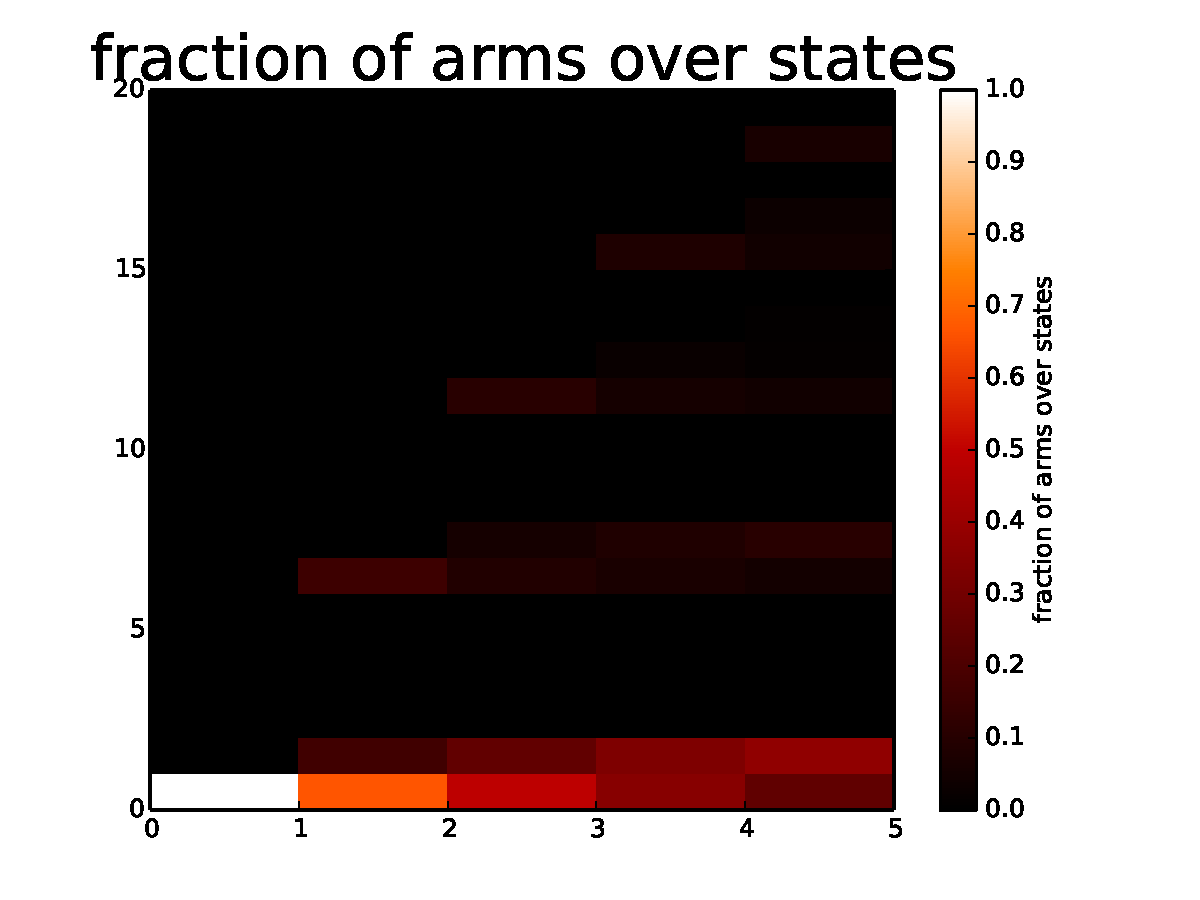
\includegraphics[width=45mm]{heat_map_index_s.pdf}}}
\only<1>{\subfigure{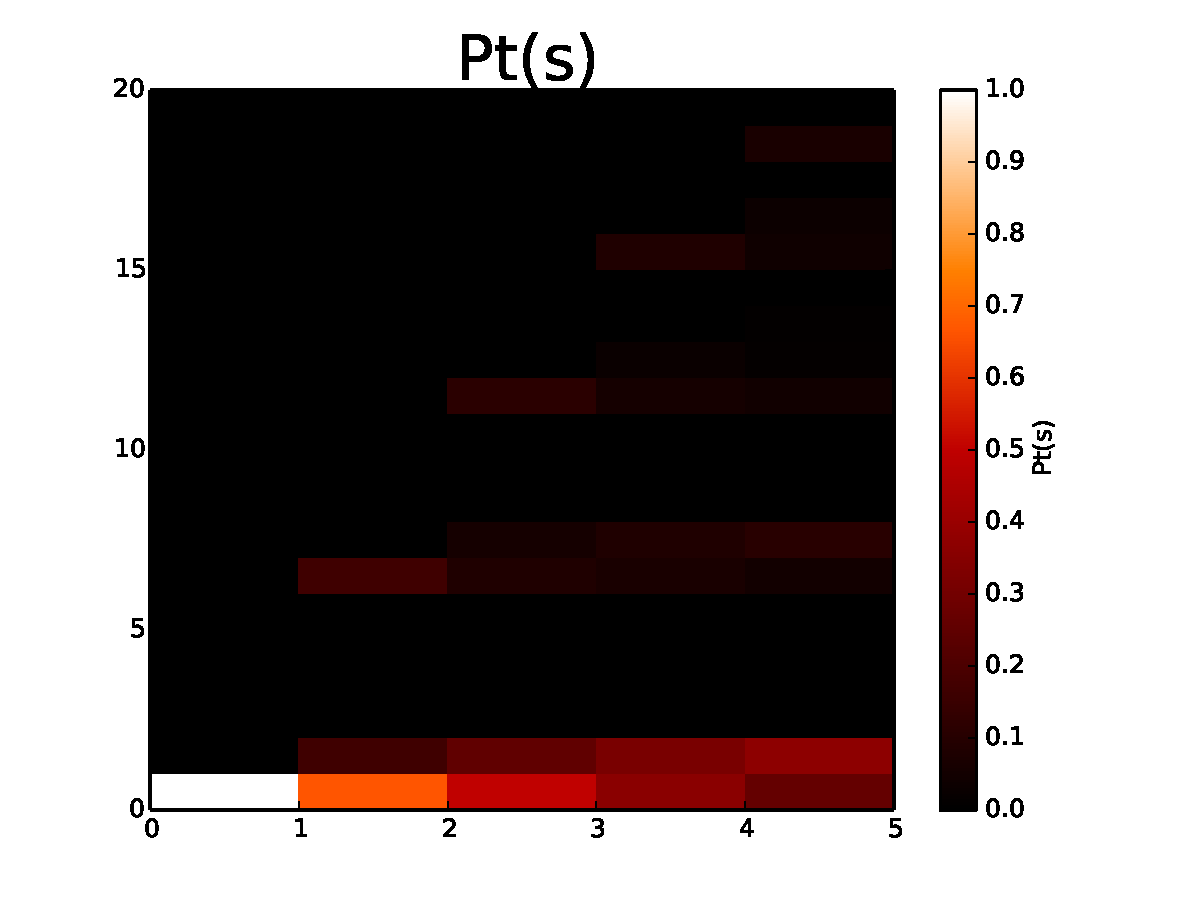
\includegraphics[width=45mm]{heat_map_pistar_s.pdf}}}
\only<1>{\subfigure{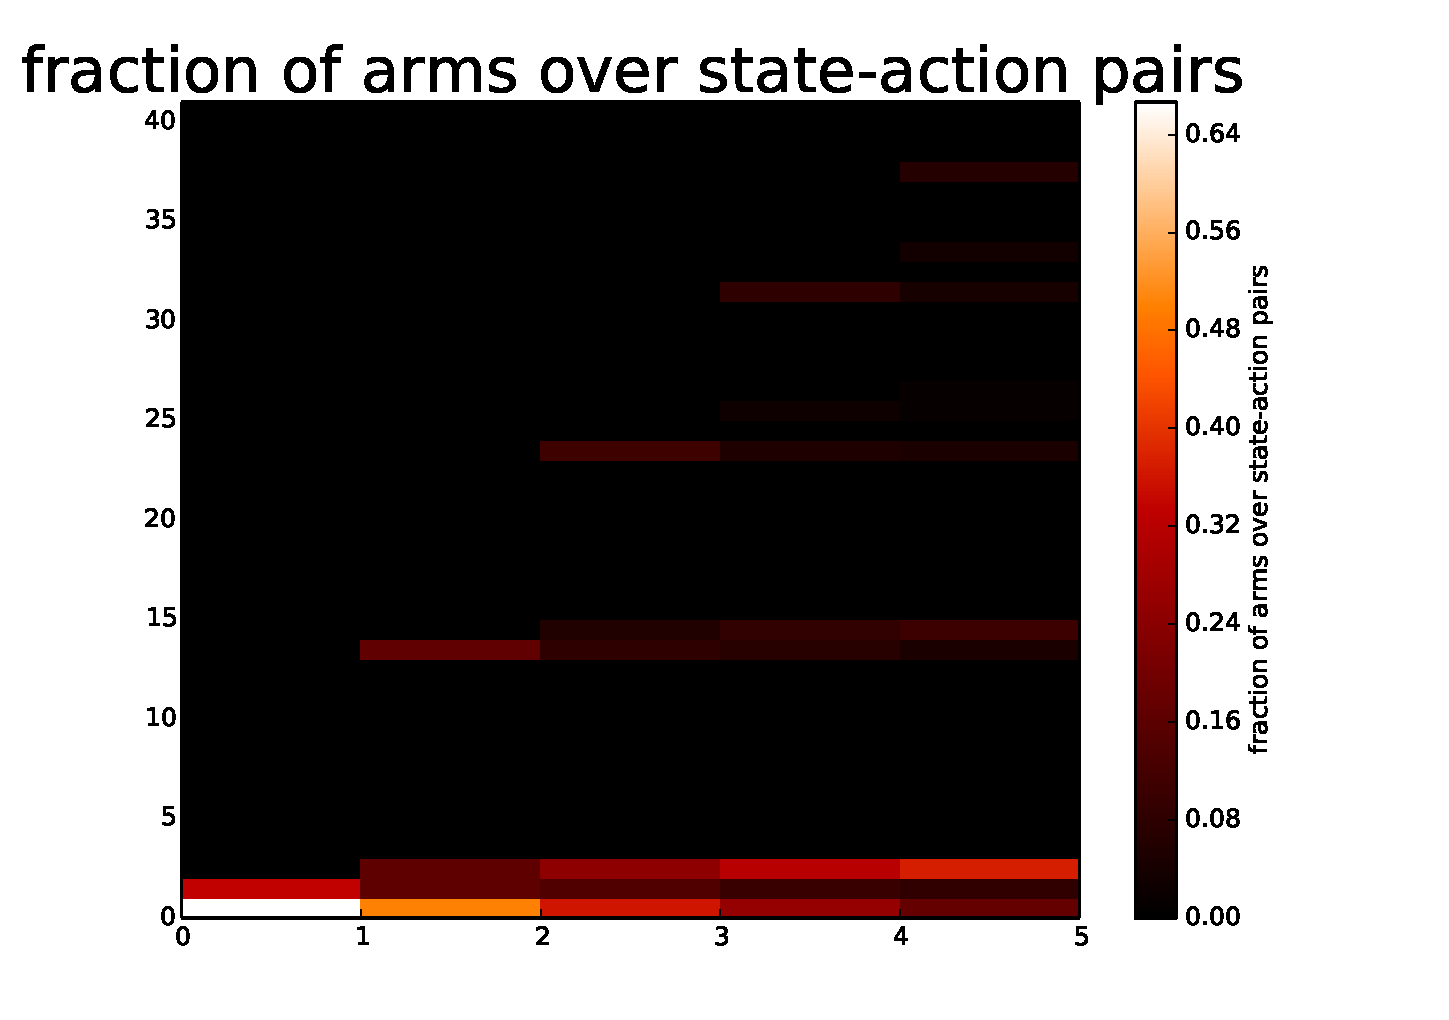
\includegraphics[width=45mm]{heat_map_index_sa.pdf}}}
\only<1>{\subfigure{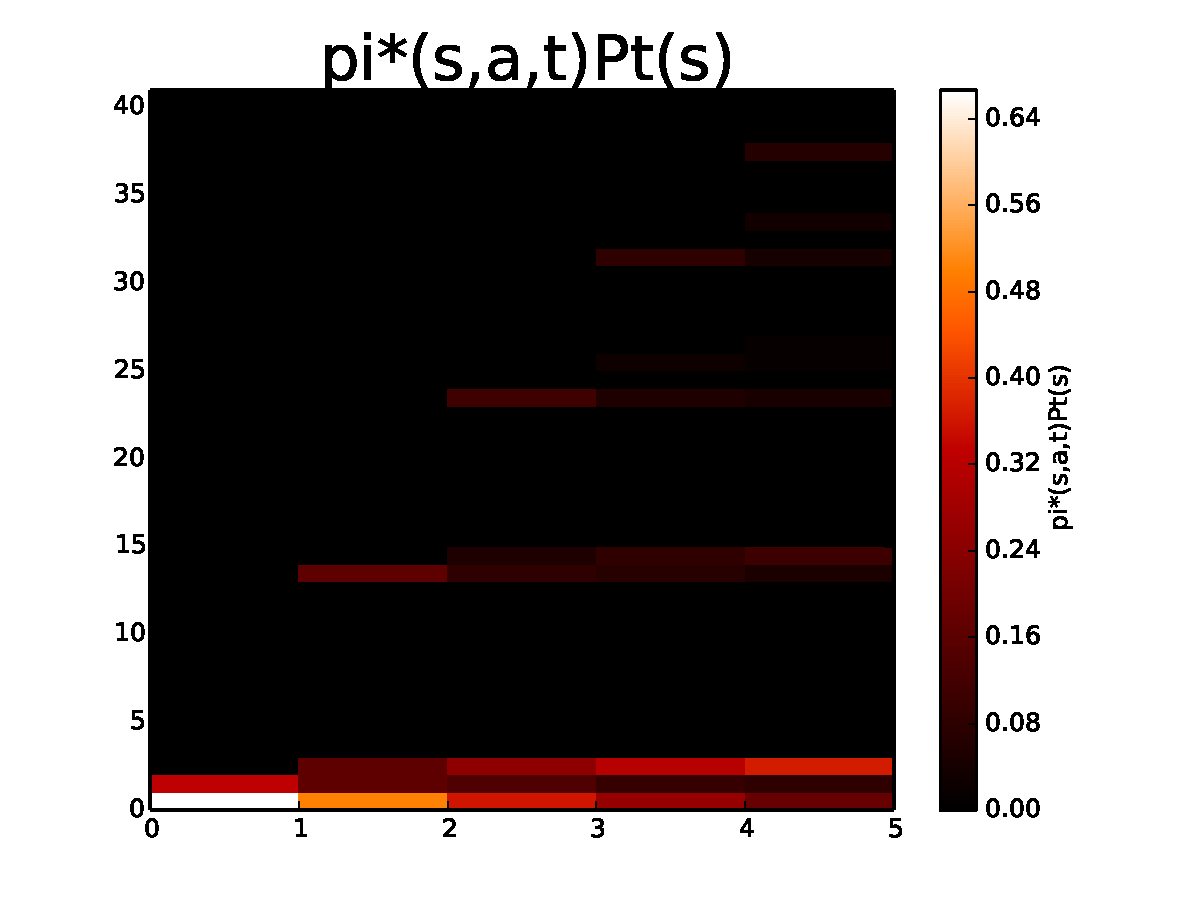
\includegraphics[width=45mm]{heat_map_pistar_sa.pdf}}}
\end{figure}
\end{frame}
%%%%%%%%%%%%%%%%%%%%%%%%%%%%%%%%%%%%%%%%%%%%%%%%

%%%%%%%%%%%%%%%%%%%%%%%%%%%%%%%%%%%%%%%%%%%%%%%%
\begin{frame}[plain]
\frametitle{Theorem 2 is proven by induction over time}
Proof Intuition of Theorem 2 (Warning: lots of hand-waves):
Assume Theorem 2 holds for time $t-1$.
\begin{itemize}
\item Proof that the first result holds at $t$:\\
Same distribution of arms over state, same fraction of arms get to set active in each state $\Rightarrow$ same distribution of arms over state in the next time period.
\item Proof that the second result holds at $t$:\\
\begin{itemize}
\item 1. $\{s\in \substates: \beta_t(s)>\lambda^*_t\}\approx \{s\in \substates: \pi^{*} \text{ chooses } a=1 \text{ in } s\}$.\\
\hspace{0.05cm}2. $\pi^{*}$ chooses $a=1$ $\alpha_t$ of the time.
\item $1 + 2\Rightarrow$ $\sum_{s\in \{s\in \substates: \beta_t(s)>\lambda^*_t\}}P_t(s)\approx\alpha_t$ \\
$\Rightarrow$  $\sum_{s\in \{s\in \substates: \beta_t(s)>\lambda^*_t\}}\frac{N_t(s)}{K}\approx\alpha_t$ .
\item The index policy $\hat{\pi}$ sets $\alpha_t K$ arms active, hence 
\end{itemize}
\end{itemize}
\end{frame}
%%%%%%%%%%%%%%%%%%%%%%%%%%%%%%%%%%%%%%%%%%%%%%%%

%%%%%%%%%%%%%%%%%%%%%%%%%%%%%%%%%%%%%%%%%%%%%%%%
%\begin{frame}[plain]
%\frametitle{Theorem 1 is proven }
%That $\hat{\allp}$ being feasible implies $$Z(\hat{\allp},\lfloor \alpha K\rfloor,K) \leq \max_{\allp\in\allpset_{\lfloor \alpha K\rfloor,K}}Z(\allp,\lfloor \alpha K\rfloor,K)$$.  Thus,
%\begin{equation*}
%\lim_{K\rightarrow\infty}\frac{1}{K}Z(\hat{\allp},\lfloor \alpha K\rfloor,K) \leq  \lim_{K\rightarrow\infty}\frac{1}{K}\max_{\allp\in\allpset_{\lfloor \alpha K\rfloor,K}}Z(\allp,\lfloor \alpha K\rfloor,K).
%\end{equation*}
%\end{frame}
%%%%%%%%%%%%%%%%%%%%%%%%%%%%%%%%%%%%%%%%%%%%%%%%%
%
%%%%%%%%%%%%%%%%%%%%%%%%%%%%%%%%%%%%%%%%%%%%%%%%%
%\begin{frame}[plain]
%\frametitle{Proof of Theorem 1 Cont'}
%On the other hand,
%\footnotesize
%\begin{align*}
%\lim_{K\rightarrow\infty}\frac{1}{K}Z(\hat{\allp},\lfloor \alpha K\rfloor,K) 
%=&\lim_{K\rightarrow\infty}\frac{1}{K}\Eb^{\hat{\allp}}\left[\sum_{t=1}^{T}\sum_{s\in\substates}r_t(s,1) M_{t}(s)+r_t(s,0) (N_{t}(s)-M_{t}(s))\right]\\
%=&\sum_{t=1}^{T}\sum_{s\in \substates}\left[r_t(s,1) \rho^*(s,1,t)+r_t(s,0) \rho^*(s,0,t) \right]\\
%&\;\;\;\;\;-\mathbb{E}^{\subp^*}\left[\sum_{t}\lambda^*_t \left(A_t-\alpha_t\right)\right]\\
%=& Q(\lambdav^*)+\alpha \sum\lambda^*_t\\
%=& \lim_{K\rightarrow\infty}\frac{1}{K}(KQ(\lambdav^*)+\lfloor \alpha K \rfloor\sum\lambda^*_t)\\
%=& \lim_{K\rightarrow\infty}\frac{1}{K} P(\lambdav^*,\lfloor \alpha K \rfloor, K)\\
%\geq& \lim_{K\rightarrow\infty}\frac{1}{K}\sup_{\allp\in\allpset_{\lfloor \alpha K\rfloor,K}}Z(\allp,\lfloor \alpha K\rfloor,K).
%\end{align*}
%\end{frame}
%%%%%%%%%%%%%%%%%%%%%%%%%%%%%%%%%%%%%%%%%%%%%%%%%

%%%%%%%%%%%%%%%%%%%%%%%%%%%%%%%%%%%%%%%%%%%%%%%%
\subsection{Numerical experiments}
\begin{frame}[plain]
\tableofcontents[currentsubsection]
\end{frame}
\begin{frame}[plain]
\frametitle{Numerical Experiments: Bernoulli MAB}
$K$ arms, each returns a random reward of 0 or 1 when pulled. $T=6$, $\alpha_t=\frac{1}{3}$, for all $t$.\\
The problem aims to maximize the total expected reward.
\begin{center}
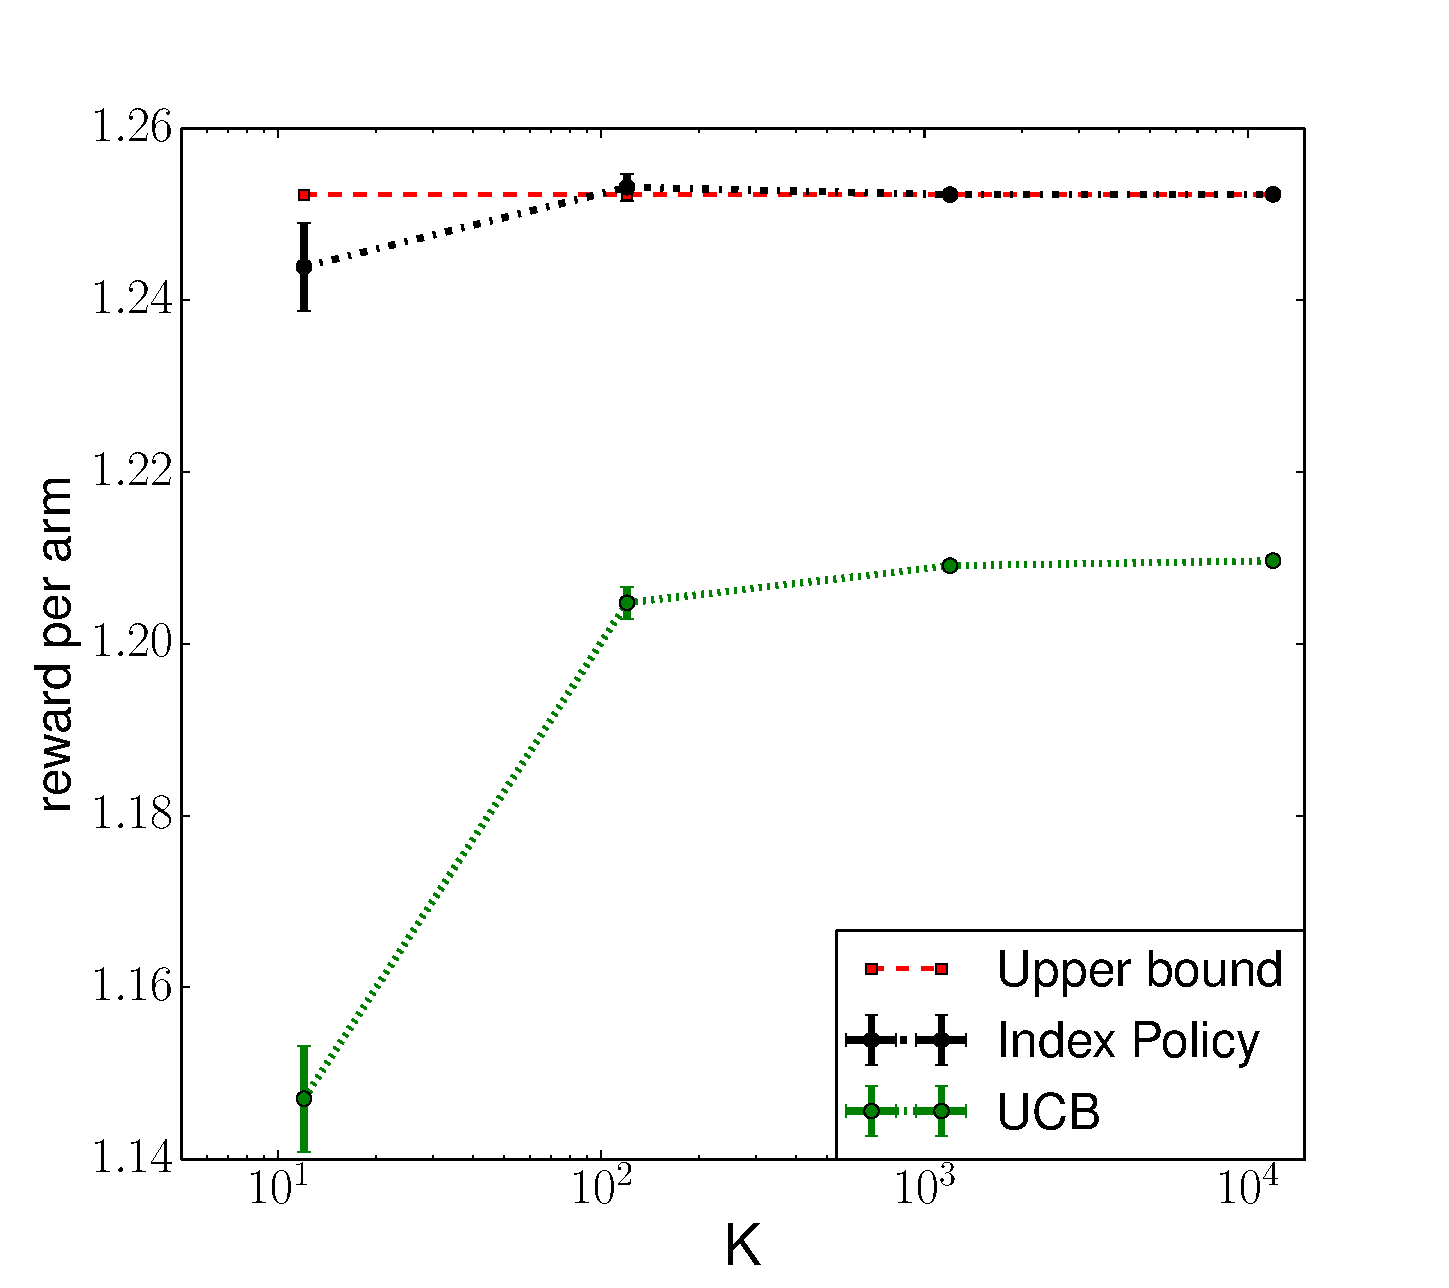
\includegraphics[width=70mm]{plot_mab.pdf}
\end{center}

\end{frame}
%%%%%%%%%%%%%%%%%%%%%%%%%%%%%%%%%%%%%%%%%%%%%%%%

%%%%%%%%%%%%%%%%%%%%%%%%%%%%%%%%%%%%%%%%%%%%%%%%
\begin{frame}[plain]
\frametitle{Numerical Experiments: Subset Selection Problem}
$K$ designs, $m$ parallel computing resources. $T=5$\\
$\alpha_t = 0.5$ for $1\leq t\leq 4$. $\alpha_5=0.3$\\
The problem aims to select the best $\bar{m}$ designs out of $K$.
\begin{center}
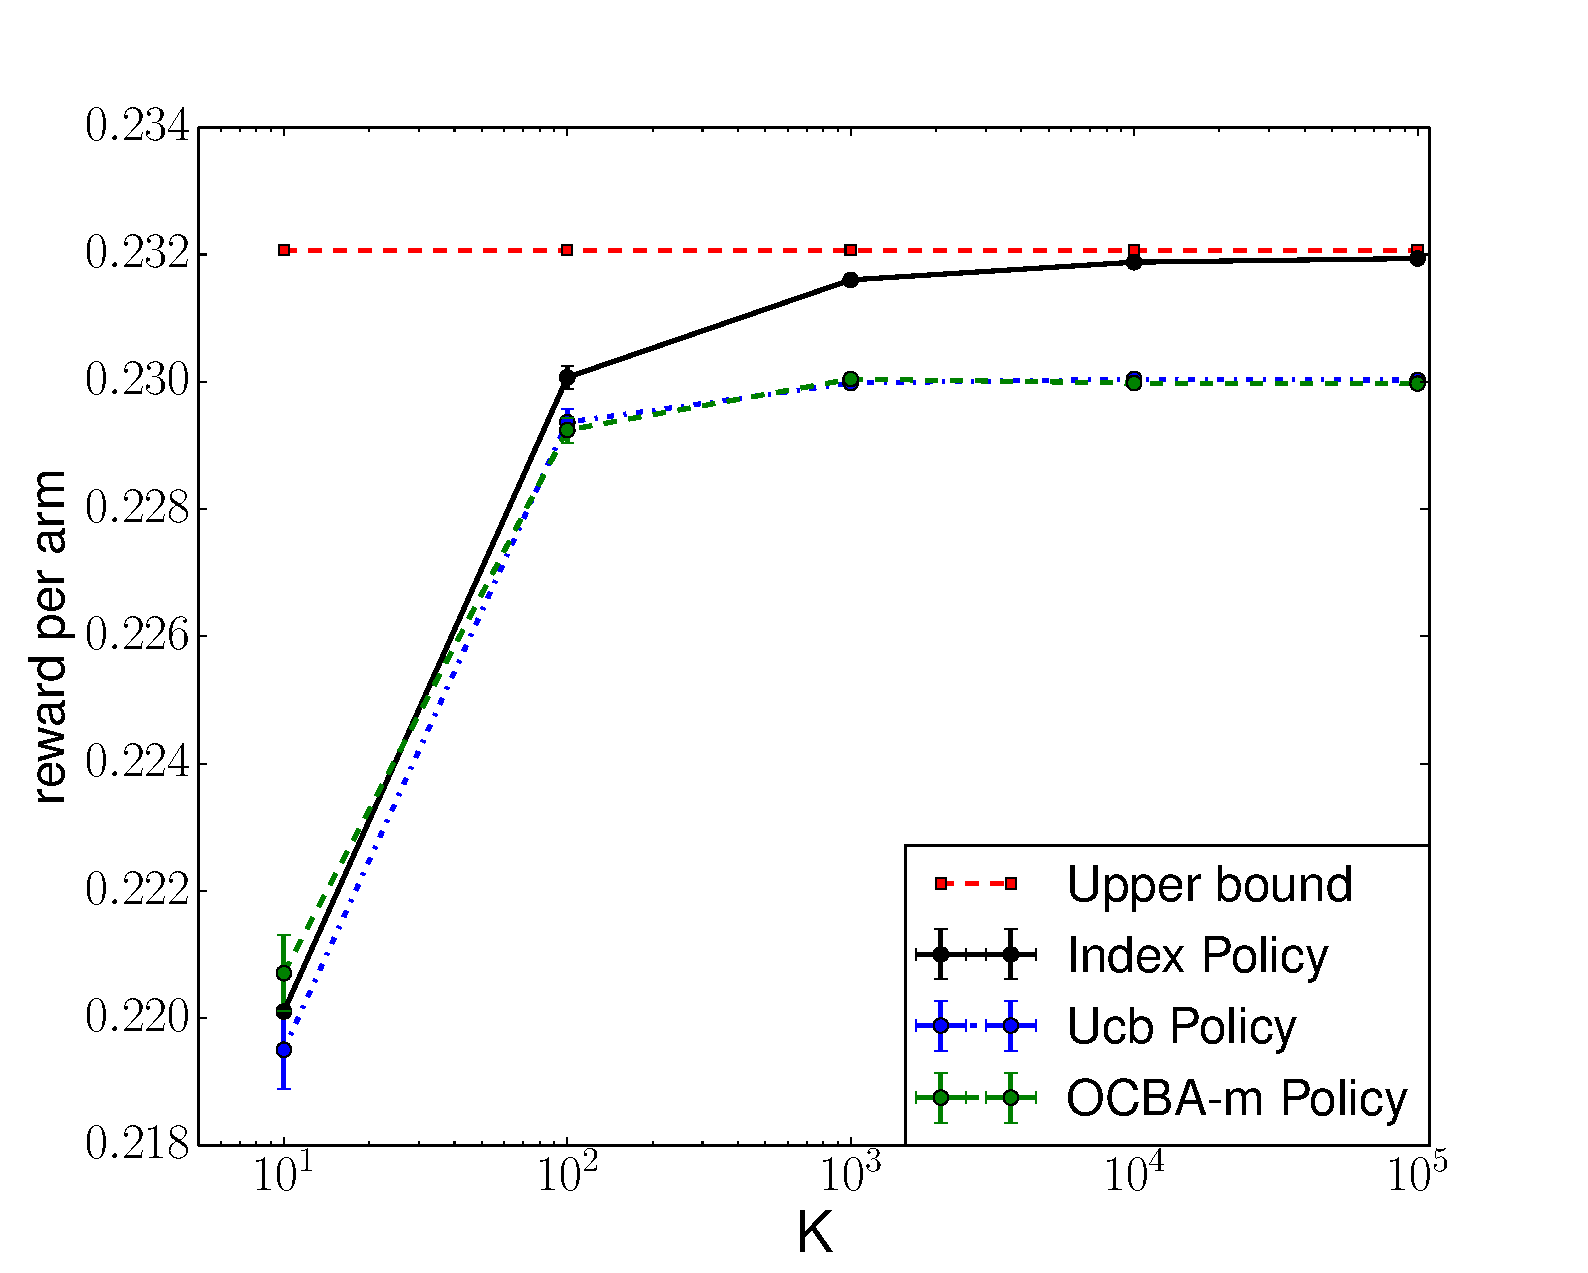
\includegraphics[width=70mm]{plot_hiring1.pdf}
\end{center}
\end{frame}
%%%%%%%%%%%%%%%%%%%%%%%%%%%%%%%%%%%%%%%%%%%%%%%%

%%%%%%%%%%%%%%%%%%%%%%%%%%%%%%%%%%%%%%%%%%%%%%%%
\section{Index policy for other RMAB-like applications}
\subsection{MCS}
\begin{frame}[plain]
\frametitle{Application 1: Multiple Selection with Standard}
\begin{itemize}
\item $k$ alternatives
\item $m$ parallel simulating resources per time step
\item $T$ time horizon
\item $\theta_x$ is the underlying true performance of alternative $x$, $x\in\{1,...,k\}$
\item $d_x$ the known threshold for alternative $x$
\item $z_{n,x}$ is the number of simulation resources to use on alternative $x$ at time step $n$. This is our allocation decision. $\sum_x z_{n,x}\leq m$
\item After time step $T$, for each alternative $x$, we decide whether $\theta_x>d_x$ based on the past results of simulation
\item We obtain a reward $R = \sum_x R_x$. $R_x$ can be a 0-1 reward or linear reward.
\end{itemize}
{\Large \color{red} Goal:Find an allocation of simulation resources to best support the decision at time T}
x\end{frame}
%%%%%%%%%%%%%%%%%%%%%%%%%%%%%%%%%%%%%%%%%%%%%%%%

%%%%%%%%%%%%%%%%%%%%%%%%%%%%%%%%%%%%%%%%%%%%%%%%
\begin{frame}[plain]
\frametitle{Application 1: Multiple Comparison with Known Standard}
For each $k=2,4,8,16$
\begin{itemize}
\item $m = k$
\item $d_x = 0.2, \forall x \in \{1,...,k\}$
\item $\Sv_0=(\alphav_0,\betav_0)=(1,1)^k$
%\item $\square$ -- Upper bound
%\item --- 95\% confidence interval with index policy, based on 10000 replications
%\item {\huge\textbf{--}}  95\% confidence interval with equal allocation policy, based on 50000 replications
\end{itemize}
\vspace{-1cm}
\begin{center}
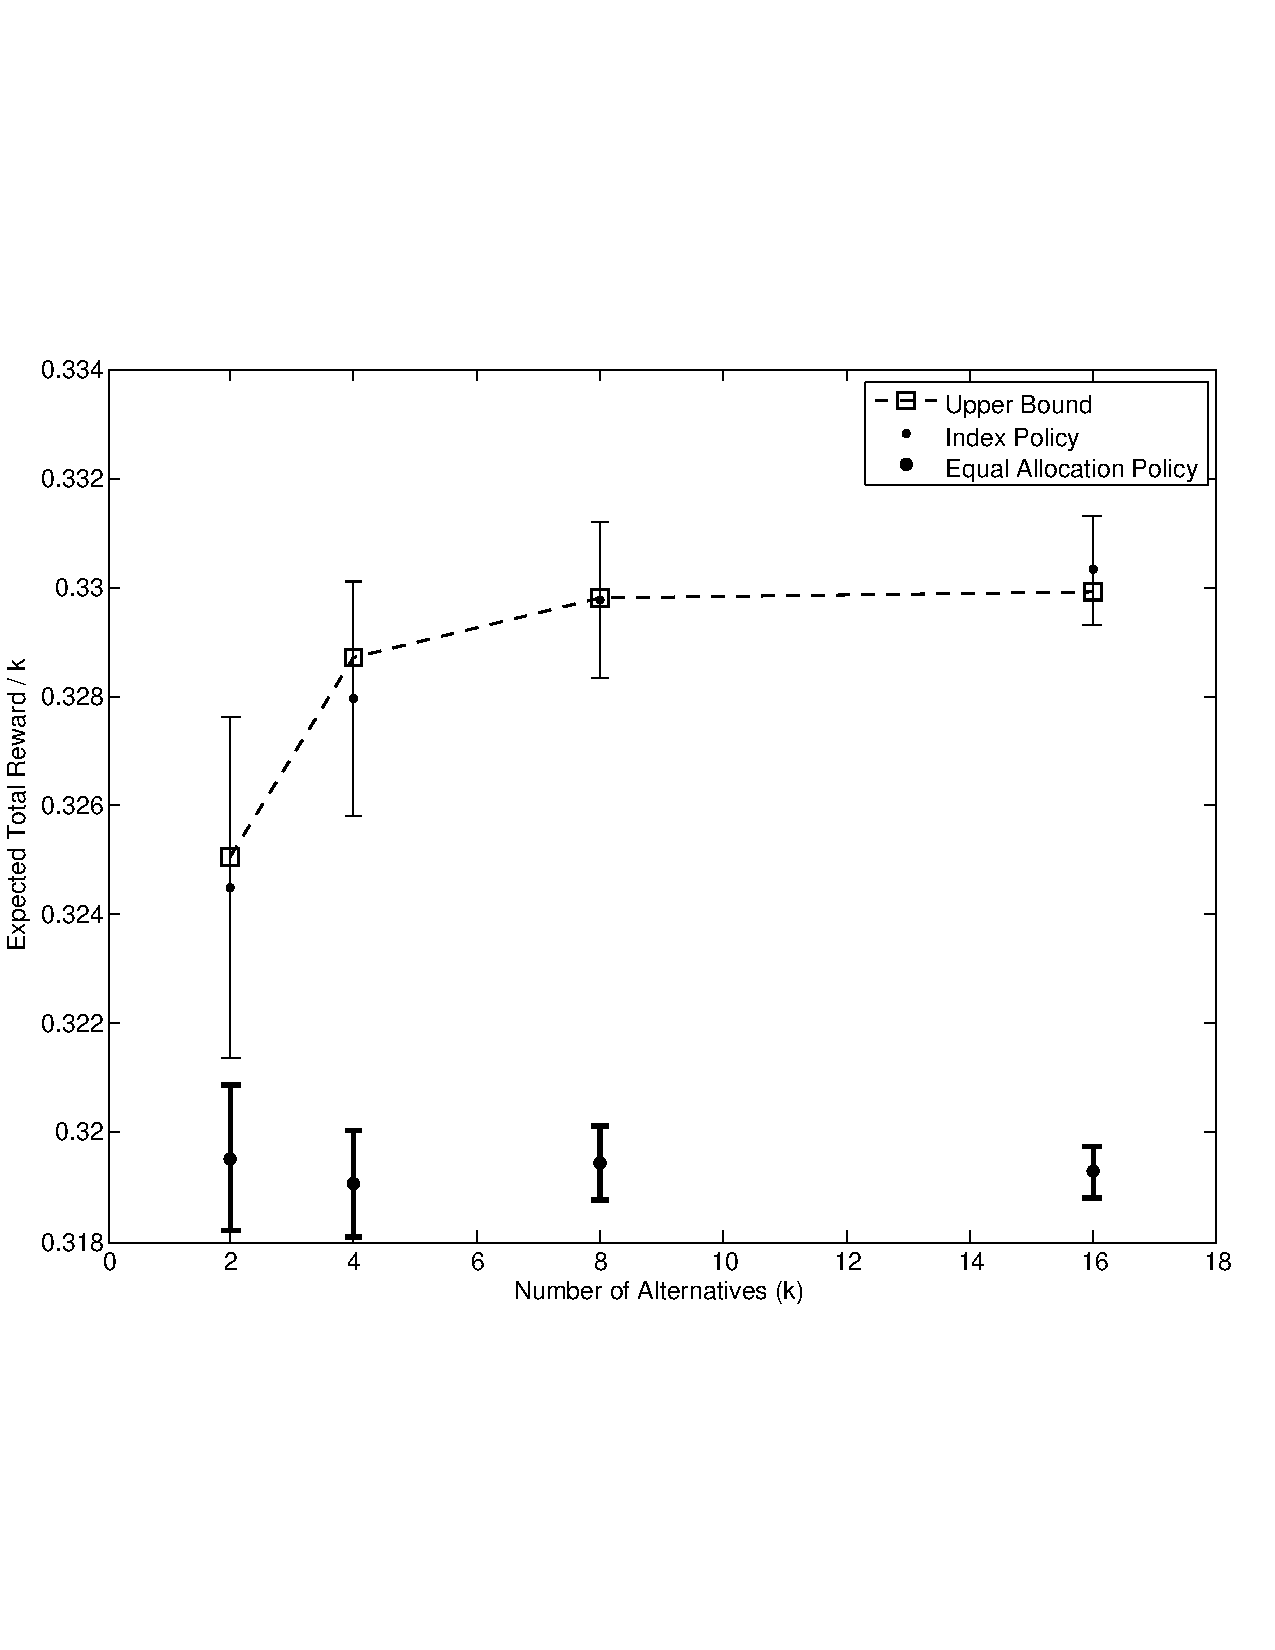
\includegraphics[width=60mm]{simPlots_0707_cropped.pdf}
\end{center}
Conjecture: The index policy has asymptotic optimality as $m$ and $K$ goes to infinity at the same rate.
\end{frame}
%%%%%%%%%%%%%%%%%%%%%%%%%%%%%%%%%%%%%%%%%%%%%%%%

%%%%%%%%%%%%%%%%%%%%%%%%%%%%%%%%%%%%%%%%%%%%%%%%
\subsection{crowdsourcing}
\begin{frame}[plain]
\frametitle{Application 2: Classification with Crowdsourcing}
\begin{itemize}
\item $k$ labeling tasks
\item $U$ total workers
\item M/M/k queue: workers come in with rate $r$, and complete their job with rate $\mu$.
\item $\theta_x$ is the underlying likelihood for a task to have a positive label.
\item $d_x$ the known threshold for alternative $x$
\item After worker budget $U$ has been exhausted, for each alternative $x$, we decide whether the true label is positive or negative based on a 1-0 reward.
\end{itemize}
{\Large \color{red} Goal:Find an allocation of workers to best support the final decision on true labels}
\end{frame}
%%%%%%%%%%%%%%%%%%%%%%%%%%%%%%%%%%%%%%%%%%%%%%%%

%%%%%%%%%%%%%%%%%%%%%%%%%%%%%%%%%%%%%%%%%%%%%%%%
\begin{frame}[plain]
\frametitle{Application 2: Classification with Crowdsourcing}
Queue: $r=0.1$, $\mu=0.4$, $K = 10,100,1000$, $U = 1.2K$. \\
We use a non-informative prior with $\alphav = \mathbf{1}$ and $\betav = \mathbf{1}$, and a threshold $d_x = 0.5$ for all the tasks. 
\begin{center}
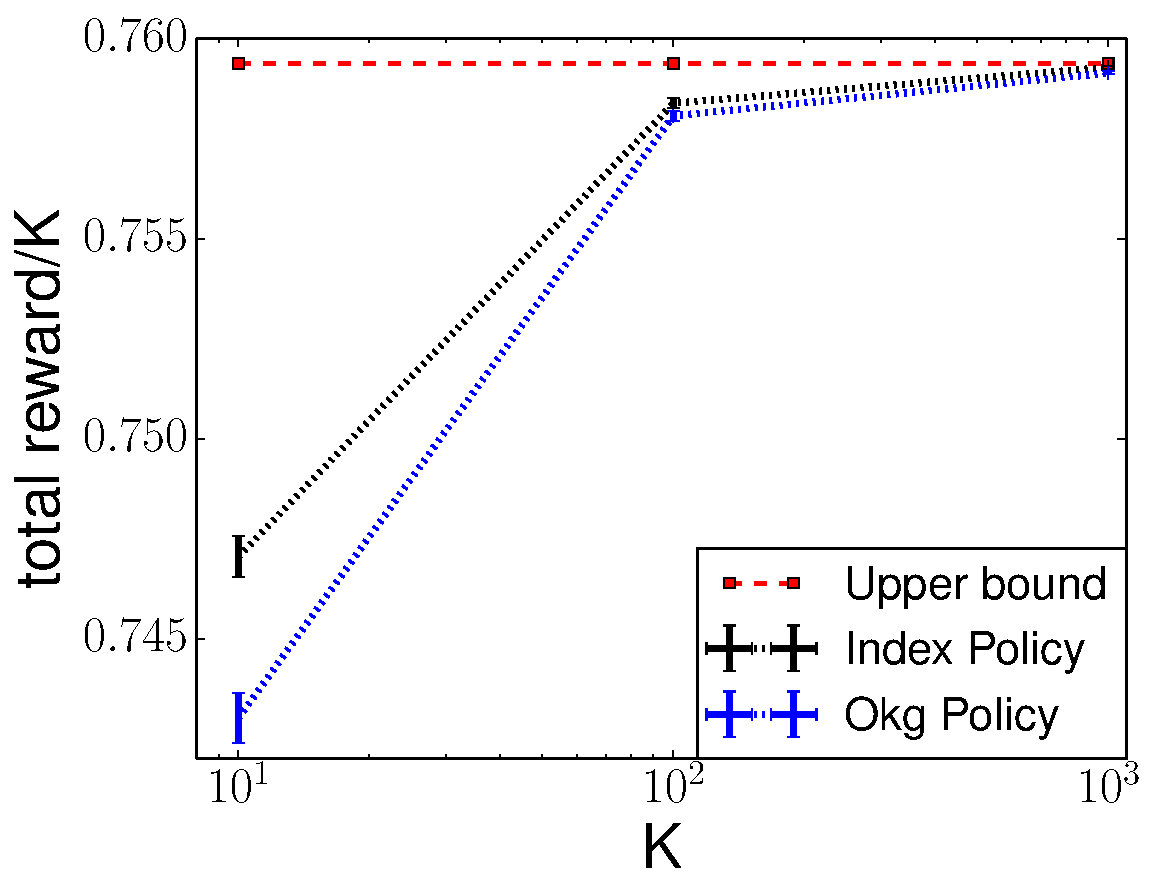
\includegraphics[width=70mm]{plot_up_sim.pdf}
\end{center}
\end{frame}
%%%%%%%%%%%%%%%%%%%%%%%%%%%%%%%%%%%%%%%%%%%%%%%%

%%%%%%%%%%%%%%%%%%%%%%%%%%%%%%%%%%%%%%%%%%%%%%%%
\begin{frame}[plain]
\frametitle{Application 2: Classification with Crowdsourcing}
We used dataset PASCAL RTE-1\cite{Snow2008}, which consists of 800 tasks, each comes with 10 labels obtained from crowdworkers and a gold standard label\\

\begin{center}
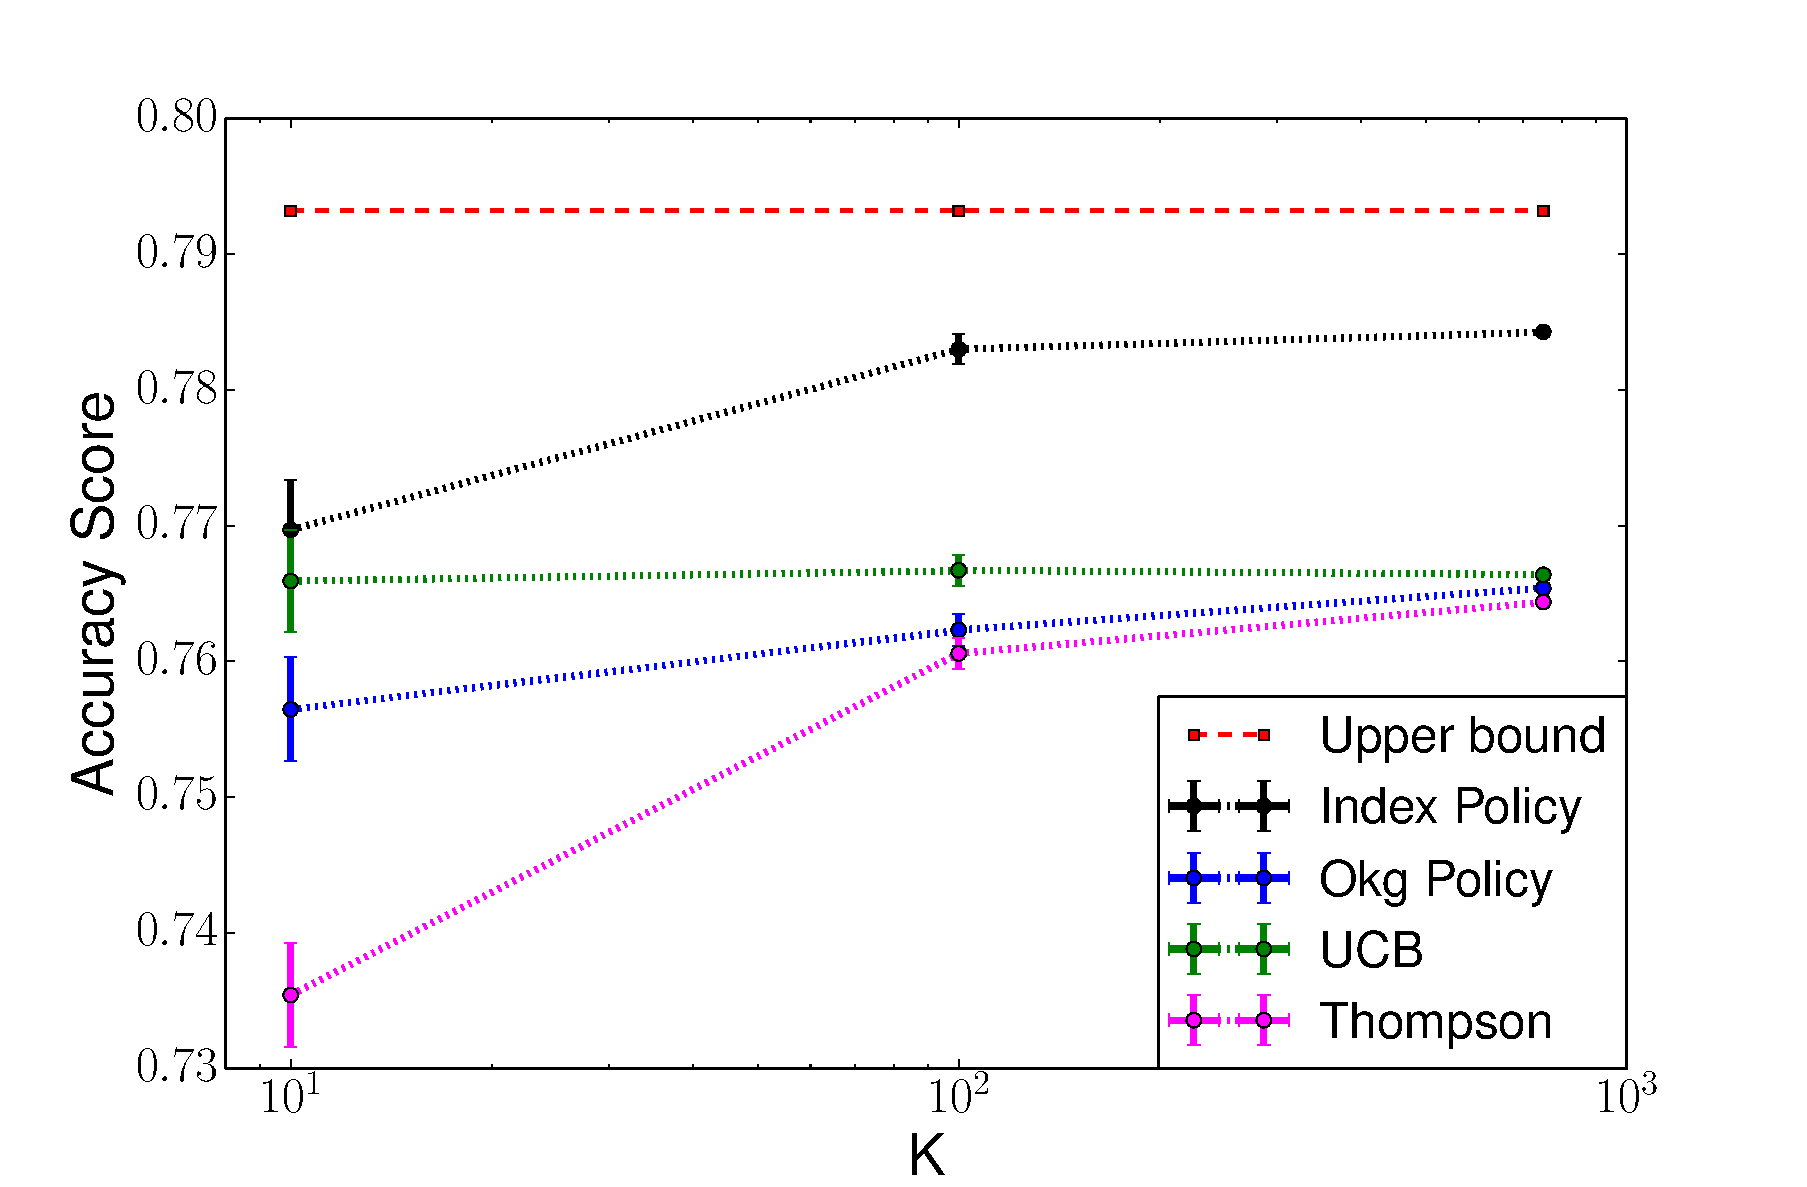
\includegraphics[width=75mm]{plot_real_sim_reward.pdf}
\end{center}

Conjecture: The index policy has asymptotic optimality as $U$ and $K$ goes to infinity at the same rate.
\end{frame}
%%%%%%%%%%%%%%%%%%%%%%%%%%%%%%%%%%%%%%%%%%%%%%%%

%%%%%%%%%%%%%%%%%%%%%%%%%%%%%%%%%%%%%%%%%%%%%%%%
\section{Conclusion}
\begin{frame}[plain]
\frametitle{Conclusion}
Index policies under different setting show asymptotically optimal behaviors while significantly reduce the computational complexity.

Possible extension of the framework:
\begin{itemize}
\item To include infinite state space
\item To allow a total budget over all time period
\item To allow multiple actions
\item To allow a more general weakly coupled dynamic program setting
\end{itemize}
\end{frame}
%%%%%%%%%%%%%%%%%%%%%%%%%%%%%%%%%%%%%%%%%%%%%%%%
\end{document}










